\documentclass[crop,tikz]{standalone}
\usepackage{amsmath}
\usepackage{amsfonts}
\usepackage{physics}
\usepackage{tikz}
\usetikzlibrary{shapes}
\usepackage{dsfont}
\usepackage{bbm}
% parameters for the MPS drawings
\definecolor{Tcolor}{RGB}{255, 235, 171}
\definecolor{Wcolor}{RGB}{190, 190, 255}
\def\textoffsetVertical{0.8}
\def\nodewidth{0.6*28.5}
\def\legwidth{0.8}
\def\nodedistance{1.25}
\def\textoffsetVerticalW{0.9}
\def\textoffsetHorizontalW{-0.9}
\def\textoffsetVerticalMPO{1.2}
\def\yoffset{1}
\def\xoffset{3}
\def\resultMPSYoffset{2.5}
\def\resultMPSXOffsetSmall{2}
\def\resultMPSXOffset{3}
\def\dotsOffset{3}
\def\conjOffsetVertical{1.25}
\def\conjOffsetVerticalLarge{2.2}
\def\curvedLineXOffset{0.7}
\def\cmscale{28.5}
\def\miniatureScale{0.5}
\def\Heffheight{1.2*28.5}
\def\Heffwidth{4.0*28.5}
\def\Heffonewidth{3.0*28.5}
\def\miniatureTextOffsetVertical{0.5}
\begin{document}
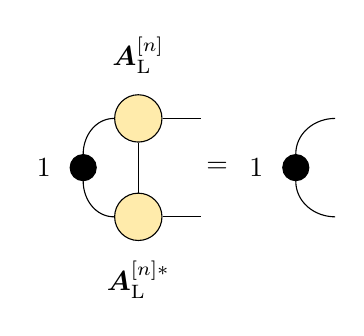
\begin{tikzpicture}[baseline=(current  bounding  box.center)]
    \node[draw, shape=circle, fill=black] (eye1) at (0, -\conjOffsetVertical/2) {};
    \node[] (eyetext) at (-0.5, -\conjOffsetVertical/2) {$\mathbbm{1}$};
    \node[draw, shape=circle, fill=Tcolor, minimum width=\nodewidth] (T) at (\curvedLineXOffset, 0) {};
    \node[] (Ttext) at (\curvedLineXOffset, \textoffsetVertical) {$\vb*{A}_\text{L}^{[n]}$};
    \node[draw, shape=circle, fill=Tcolor, minimum width=\nodewidth] (Tc) at (\curvedLineXOffset, -\conjOffsetVertical) {};
    \node[] (Ttext) at (\curvedLineXOffset, -\conjOffsetVertical-\textoffsetVertical) {$\vb*{A}_\text{L}^{[n]*}$};
    \draw (eye1) to[in=180, out=90, looseness = 1] (T);
    \draw (eye1) to[in=180, out=-90, looseness = 1] (Tc);
    \draw (T) -- (Tc);
    \draw (T) -- ++(\legwidth, 0);
    \draw (Tc) -- ++(\legwidth, 0);

    \node[] (equalsign) at (\resultMPSXOffsetSmall/2+\curvedLineXOffset, -\conjOffsetVertical/2) {$=$};

    \node[draw, shape=circle, fill=black] (eye) at (\resultMPSXOffsetSmall+\curvedLineXOffset, -\conjOffsetVertical/2) {};
    \node[] (eyetext) at (\resultMPSXOffsetSmall-0.5+\curvedLineXOffset, -\conjOffsetVertical/2) {$\mathbbm{1}$};
    \draw (eye) to[in=180, out=90, looseness = 1] ++(0.5, \conjOffsetVertical/2);
    \draw (eye) to[in=180, out=-90, looseness = 1] ++(0.5, -\conjOffsetVertical/2);
\end{tikzpicture}
\end{document}